%TEX root = ../dissertation.tex

\chapter{State of the art}
\label{chapter:state-of-the-art}
%
% SDN
\section{Software-Defined Networking}
\label{section:software-defined-network}
\gls{SDN} relies on two fundamental changes to the current networking concept in order to solve the management issues of traditional networks mentioned in Chapter \ref{chapter:introduction}: the decoupling of network control and forwarding planes and network programmability\cite{OFWP}.
% 
Traditional network nodes are built of the basis of a three strongly-coupled planes of functionality architecture.
These are the \emph{management plane}, which allows for service monitoring and policy definition, the \emph{control plane}, which enforces the policies in network devices and the \emph{data plane} which efficiently forwards data.
Figure \ref{fig:Traditional_Network_Architecture} depicts a two node network according to this approach to networking architecture.\\
\begin{figure}
	\centering
	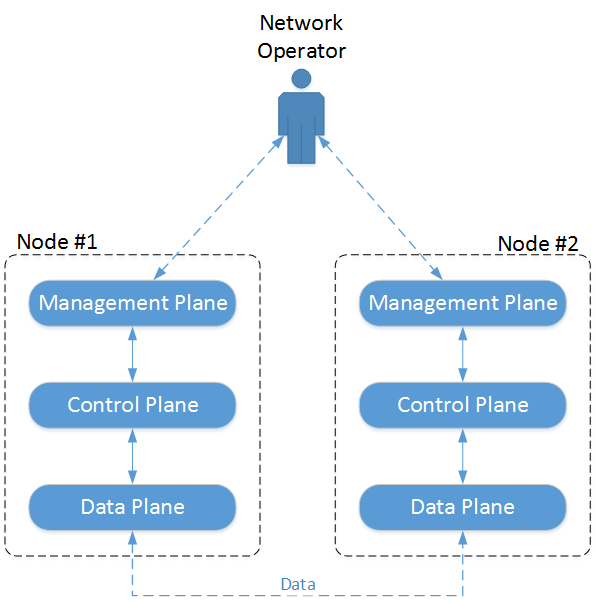
\includegraphics[scale=0.65]{Traditional_Network_Architecture}
	\caption{Two node network according to the traditional network node architecture.}
	\label{fig:Traditional_Network_Architecture}
\end{figure}
%
Having these three planes tightly-coupled and implemented in the network nodes is the reason behind both the box-centric configuration style and vendor-specific configuration workflow and interface.
\gls{SDN} decouples these planes from one another, defining the abstraction of \emph{Specification}, corresponding to the management plane functionality, \emph{Distribution}, corresponding to the control plane functionality, and \emph{Forwarding}, corresponding to the data plane functionality.
By doing so, this new architectural concept makes it possible to logically centralize the \emph{Specification} and \emph{Distribution} while keeping the \emph{Forwarding} implemented in the network nodes\cite{Kreutz2014}\cite{OFWP},\cite{OpenNetworkingFoundation} thus creating the premises for a network infrastructure that harnesses the benefits of both distributed data forwarding and centralized management, dismissing today's decentralized network management style.\\
%
The second core feature of \gls{SDN} is the ability to programmatically configure the network, which is accomplished by having the Specification expose a set of \glspl{API} to be consumed by network applications.
These \glspl{API} are generally capable of exposing the network topology through global and abstracted views, as well as providing methods of global policy definition and common network functionality such as routing, access control and bandwidth management\cite{OFWP}.
The policies are then applied to the appropriate network nodes by the \emph{Distribution} through the use of a communication protocol implemented both on this abstraction and on the network elements.\\
%
These two core concepts lead to the definition of the architecture of \gls{SDN} in three layers, the \emph{Application} layer, the \emph{Control} layer and the \emph{Infrastructure} layer \cite{OpenNetworkingFoundation}\cite{Kreutz2014} as depicted in Figure \ref{fig:SDN_Architecture}.
\begin{figure}
	\centering
	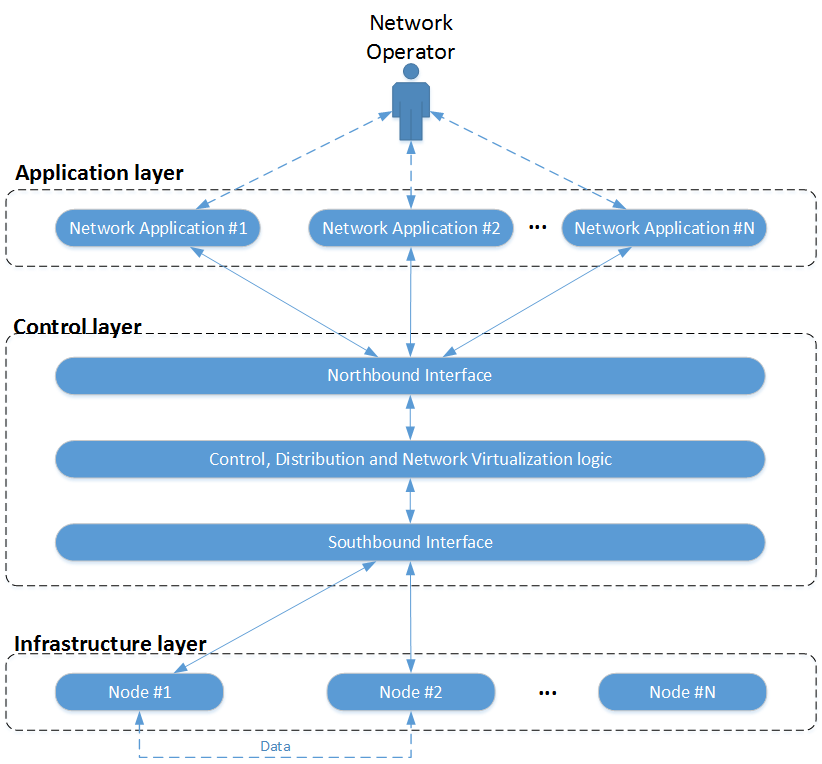
\includegraphics[scale=0.70]{SDN_Architecture}
	\caption{Two node network according to the SDN architecture.}
	\label{fig:SDN_Architecture}
\end{figure}
The Infrastructure layer is where all the network nodes reside, performing all the Forwarding functions.
The Control layer encompasses the Specification and the Distribution, therefore dealing with all the network management and control mechanisms.
The Application layer is where the network applications reside.
These applications define the network policies through the Control's northbound \glspl{API}, taking into account factors such as (but not restricted to) network topology and the network operator input.\\
This three-layered architecture, depicted in figure \ref{fig:SDN_Architecture}, is commonly extended to a for-layered architecture by breaking the Control layer in two, creating a layer solely for network virtualization that sits between the Control and Infrastructure layers.\\
%
The implementation of the Control layer is known as \gls{SDN} controller or \gls{NOS}, and it is the main building block for Software-Defined Networks.
A \gls{SDN} Controller exposes a northbound interface, intended for interaction with network applications corresponding to the Specification functionality, a southbound interface intended for interaction with the network elements in the scope of the Distribution functionality, and in some cases eastbound/westbound interfaces for integration with other \gls{SDN} controllers (mostly seen in distributed controllers)\cite{Kreutz2014}.
The southbound interface must implement the same protocol as network elements do in order for network programmability to work, effectively making the definition of good standard protocols and acceptance of said protocol by vendors a key point of action for \gls{SDN} to prosper.\\
%
By comparing figures \ref{fig:Traditional_Network_Architecture} and \ref{fig:SDN_Architecture} it is easy to understand that this new architecture simplifies management by having it done in a single point (Control layer) instead of multiple points (network nodes) and fosters innovation as the implementation of new network policies or custom network behavior can now be promptly implemented by introducing an application to do so without the need of knowing how it will be implemented in the network infrastructure or even of how the network infrastructure is composed.
Furthermore, applications can be written to dynamically adjust network policies according to the network status without the need for Human intervention, thus drastically reducing the time required to adjust network policies upon network events such as topology changes and therefore potentially increasing the effectiveness of said policies should the event pose a security threat or risk of service outage.
Another inherent advantage of this solution is the consistency of the policy throughout the network, seeing that the policy is now defined by the network operator through a network application in a global scope and in a single point, therefore eliminating inconsistencies in configurations between different network nodes.\\
%

There are currently several implementations for SD\gls{SDN}N controllers such as OpenDaylight\cite{OpenDaylight}, Floodlight\cite{Floodlight} and ONOS\cite{ControllerComparison} \cite{Kreutz2014}, as well as southbound interfaces such as OpenFlow, POF, ForCES and OpFlex \cite{Kreutz2014}.
Although at first it might not be obvious at first, the fact that multiple southbound interfaces exist presents itself as an issue, given that either network elements or \gls{SDN} controllers must implement more than one of them in order to achieve compatibility between \gls{SDN} controllers and network elements.
Because there is now a dominant southbound interface - OpenFlow - the vast majority of network elements implementing the \gls{SDN} architecture are implementing only OpenFlow.\\
%
The \gls{ONF} has made OpenFlow a standard protocol and is working on standardizing the northbound interfaces\cite{OFWP}, which will make network applications controller-agnostic, which in turn will streamline development and make application portability possible.\\
%
Today's data center's multitenancy is growing as a consequence of \gls{IaaS} and as such infrastructure virtualization becomes increasingly important both for security and service reasons.
With more and more companies migrating their \gls{IT} infrastructure to private cloud infrastructures, network virtualization starts to gain new perspectives as traffic isolation is not enough, with support for custom tenant network topologies being required to smooth the transition.
There are also several network virtualization implementations for \gls{SDN} such as FlowVisor\cite{Sherwooda}\cite{Sherwood} and OpenVirteX\cite{Kreutz2014}.
These implementations are analogous to the hypervisors in \gls{IT} virtualization, sitting between the \gls{SDN} controller and the network elements, acting as a proxy for the communications between both.
Multiple \gls{SDN} controllers are allowed to interact with the same instance of the virtualization layer, one for each virtual network.\\
%
\subsection{Southbound interfaces}
\label{subsection:sdn-southbound-interfaces}
The \gls{SDN} architecture is possible due to the existence of protocols for programming the forwarding plane, also referred to as southbound interfaces (from a \gls{SDN} controller perspective).
There are currently several protocols, such as \gls{POF}\cite{POF}, \gls{ForCES}\cite{ForCES}, OpFlex\cite{OpFlex} and OpenFlow\cite{OFWP}.
%
\gls{POF} attempts to enhance the forwarding plane programmability by defining generic matching rules that make use of offset definitions instead of packet header definitions.
In practice, matching in \gls{POF} is performed against a sequence of bits with specified length in a packet starting at a given position, effectively allowing the definition of matches against any packet header regardless of the protocol\cite{POF}.
%
\gls{ForCES}, despite also aiming at decoupling control from forwarding, does not require the existence of a network controller and instead the control is allowed to remain in the network nodes\cite{Kreutz2014}.
%
OpFlex mixes concepts from both OpenFlow and \gls{ForCES}, having the management being centralized while the control remains distributed in the network elements \cite{Duffy2014}.\\
%

OpenFlow, the most prominent of them, is a standard protocol for forwarding plane programming, defined by the \gls{ONF} and designed for Ethernet networks\cite{OFWP}.
It is analogous to the Instruction Set of a \gls{CPU} in the sense that it defines primitives that can be used by external applications to program the network node much like it is done with \glspl{CPU}\cite{OFWP}.
Forwarding decisions are based in the notion of flows, which according to the \gls{IETF} is "a sequence of packets from a sending application to a receiving application"\cite{IETFFLOW}.
OpenFlow is supported by several vendors such as Cisco\cite{CISCOOF}, Juniper\cite{JUNOSOF}, HP\cite{HPVAN} and Alcatel-Lucent\cite{ALUOF}.\\
%
%*** OVSDB vs OF-CONFIG
While the OpenFlow protocol allows for forwarding plane programming, some network management aspects are not entirely bound to forwarding decisions.
Some of these aspects include turning network ports on and off and establishing tunnels between network elements.
There are however other southbound protocols that introduce these management capabilities and rely on OpenFlow to implement forwarding plane programming, namely the \gls{OVSDB} and the \gls{OF-CONFIG}\cite{OVSDBvsOFCONFIG}.
\gls{OVSDB} is a component of Open vSwitch and it is designed to manage Open vSwitch implementations.
\gls{OF-CONFIG} is defined by the \gls{ONF} specifically to be used alongside with OpenFlow and may be implemented in both software or hardware network element implementations.
%
%
% OF
\section{OpenFlow}
\label{section:openflow}
Having had several versions released since 2008 when version 0.8.0 debuted, OpenFlow is currently on version 1.5\cite{OF15}.
However, because changes made from version 1.3 to version 1.5\cite{OF15}\cite{OF13} are not relevant to the scope of this work and because both hardware and software switch implementations mainly implement version 1.3 we will focus on version 1.3 for the purpose of this work.\\
%
As previously mentioned, there are now several available implementations of OpenFlow-enabled network elements, however OpenFlow implementation and traditional forwarding planes implementations are not mutually exclusive, thus the definitions of \emph{OpenFlow-only} network elements (which implement only the OpenFlow forwarding plane) and \emph{OpenFlow-hybrid} network elements (which implement both the OpenFlow and legacy forwarding planes).
In the later, OpenFlow specifies means of forwarding traffic from the OpenFlow forwarding plane and into the legacy forwarding plane\cite{OF13}.
This is in fact a major upside to OpenFlow adoption, as it makes the adoption of OpenFlow by hardware vendors as easy as releasing a new software version that implements the OpenFlow forwarding plane on top of existing network hardware, and allows adopters to gradually roll-out OpenFlow in existing networks possibly with existing network hardware.\\
%
The OpenFlow specification defines the architecture of an OpenFlow switch implementation in three main building blocks: the \emph{OpenFlow Channel}, the \emph{Processing Pipeline} and the \emph{Group Table} as depicted in figure \ref{fig:OF_switch_arch}.
\begin{figure}
	\centering
	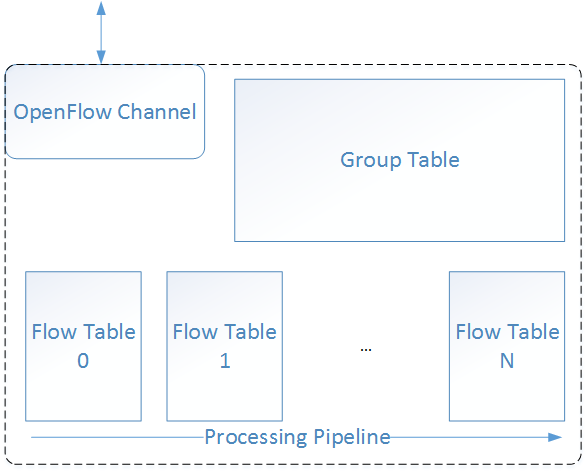
\includegraphics[scale=0.65]{OF_switch_arch}
	\caption{OpenFlow switch architecture.}
	\label{fig:OF_switch_arch}
\end{figure}
The \emph{OpenFlow Channel} defines the interface for communications between the OpenFlow switch and the \gls{SDN} controller, through which controllers can statically or dynamically create, modify and remove \emph{flow entries} from \emph{flow tables}.
Further detail on the differences between static and dynamic flow entry programming will be addressed later in this document.
All communications between an OpenFlow switch and an \gls{SDN} controller are encrypted by default using \gls{TLS} even though it is possible use plain \gls{TCP}\cite{OF13}.
These communications are always initiated by the OpenFlow switch, and each switch may have one or more \gls{SDN} controller \gls{IPAddress} specified in its base configuration.
The OpenFlow switch is required to maintain active connections witch all configured \gls{SDN} controllers simultaneously. Because multiple \gls{SDN} controllers may be configured in a single switch, each controller is assigned one of three possible roles: \emph{Master}, \emph{Slave} or \emph{Equal} \cite{OF13}.\\
The Master role grants the \gls{SDN} controller full management access to the switch, allowing it to program flow entries and receive notifications of events occurring on the switch, such as flow entries expiring and port status updates.
There can be at most one \gls{SDN} controller configured as master per switch.
The Slave role grants the \gls{SDN} controller with read-only access to the switch, allowing it to receive only port status updates.
Any \gls{SDN} controller instance that is already connected to the switch can request to change role from slave to master, at which point the instance that previously held the master role will be updated to the slave role.
This mechanism provides a fault tolerance mechanism by allowing for the existence of Active-Standby \gls{SDN} controller clusters. 
The Equal role is essentially the same as the Master role, with the exception of allowing one switch to be connected to multiple \gls{SDN} controllers in Equal role.
This specific role aims at introducing a mechanism for fault tolerance but also load balancing, requiring however that the \gls{SDN} controllers coordinate with each-other.\\
The \emph{Processing Pipeline} is composed of several \emph{flow tables} (with a required minimum of one), each containing a set of \emph{flow entries}.
A \emph{Flow entry} is defined by a set of fields, namely:
\begin{itemize}
	\item \textbf{Priority}, which defines its precedence over other flow entries in the same table, with the highest value taking precedence
	\item \textbf{Match fields} consisting of header patterns that when positively matched against a packet identify a flow
	\item A set of \textbf{instructions} that determine the course of action the switch should take to handle the flow
	\item \textbf{Timeouts} defining for how long the flow entry is to be maintained in the flow table, namely a \emph{hard timeout} which forces the flow entry to be removed $\Delta$ seconds after it was installed and a \emph{soft timeout} specifies for how long the flow entry shall be kept after the last matching packet as been matched
	\item \textbf{Counters} that increment each time a packet is successfully matched against the flow entry
	\item \textbf{Cookies}, which are used exclusively by the \gls{SDN} controller to annotate the flow entry
\end{itemize}
%
For each flow table there might be one special flow entry that matches all packets and with a priority of zero, called the \emph{table-miss flow entry} and it defines the default action set to be taken by the switch for any given packet.
Flow matching is performed in a one way direction, starting in flow table \emph{0} (which is the only mandatory flow table) and ending with either a set of actions to be executed (defined by matching entries) or alternatively dropping the packet.
This means that once processing has reached table \emph{n}, it can then either resume processing in table \emph{m} where \emph{m $>$ n} if the matching flow entry defined such instruction, or execute the actions in the instruction set defined by matching entries in tables \emph{0} through \emph{n}.
If no entries that match the packet occurred then either there is a table-miss flow, usually redirecting the packet to the \gls{SDN} controller or simply resuming the pipeline processing in the next table, or the switch drops the packet completely.
%
Last but not least, the \emph{Group Table} contains \emph{group entries}.
\emph{Group entries} allow the definition of \emph{action buckets}, which are defined by a \emph{Group Identifier} uniquely identifying the group entry, a \emph{Group Type} defining the behavior of the Group entry, and a set of \emph{Action Buckets} which are themselves sets of actions to be executed by the switch.
\emph{Group entries} are somewhat analogous to action macros, simplifying forwarding functions such as broadcast and multicast\cite{OF13}.\\
%
An OpenFlow switch may also implement a \emph{meter table} allowing for the implementation of simple \gls{QoS} features such as queue management and rate limiting\cite{OF13}.\\
The aforementioned mechanisms grant OpenFlow the ability to perform highly granular control over how specific flows should traverse the network, enabling the differentiation of traffic according to its profile\cite{OFWP}.
Consequently, network protocol implementations on network elements become increasingly deprecated, leading to the dismissal of said implementations in favor of OpenFlow forwarding plane implementations instead, thus having for the forwarding decisions being programmed from the \gls{SDN} controller according to the global policies set for the network\cite{OFWP}.\\
%
% OF Flow programming
\subsection{OpenFlow flow programming}
\label{subsection:openflow-flow-programming}
% Static vs Dynamic flows
%
\begin{figure}
	\centering
	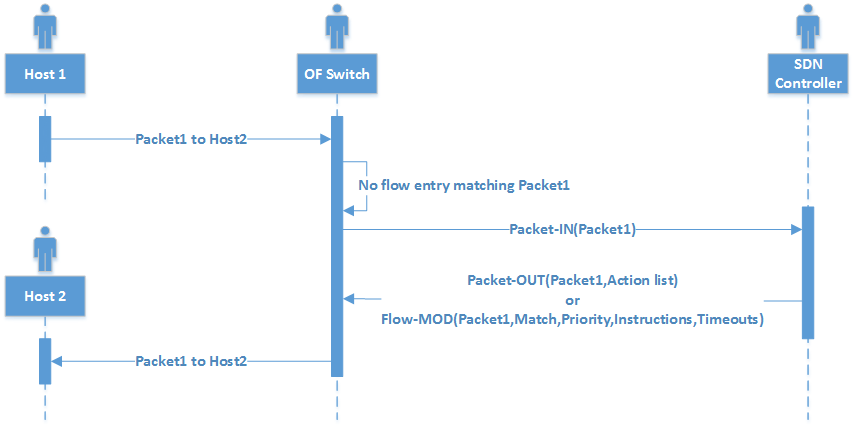
\includegraphics[scale=0.65]{OF_dynamic_flow_programming}
	\caption{OpenFlow reactive flow programming}
	\label{fig:OF_dynamic_flow_programming}
\end{figure}
%
\gls{SDN} controllers may program flow entries in OpenFlow switches by issuing \emph{flow table modification} messages.
These messages allow the \gls{SDN} controller to manipulate flow tables by adding new flow entries and modifying or removing existing flow entries.
Flow entry additions performed by the \gls{SDN} controller by issuing a flow table modification message to predefine the forwarding behavior ahead of data transmission is referred to as static flow entries and configures the proactive flow programming paradigm.
These flow entries usually have both their hard and soft timeouts set to zero, meaning that they will not expire\cite{OF13}.
Having these flow entries present in the flow tables enable the traffic to be forwarded immediately when reaching the OpenFlow switch.
However, it has the disadvantages of having to preprogram flow entries to cover every single flow possible according to the global network policy, which leads to a quick exhaustion of the flow tables available in the switch.
Furthermore, the action set being preprogrammed might not be optimal for a particular flow being processed at a particular point in time.
A typical usage of static flow entries are the table-miss flow entries, which have already been discussed.
%
Table-miss flow entries, defining an instruction to forward the packet to the \gls{SDN} controller through a \emph{packet-in} message, on the other hand enable the \gls{SDN} controller to examine the packet and define the proper actions to be executed by the switch in a reactive fashion.
The \gls{SDN} controller may respond to this message with either a \emph{packet-out} message defining the actions to be executed exclusively for that packet or alternatively with a flow table modification message that will create a new flow entry to handle all the packets matching that flow, including the original packet included in the packet-in message\cite{OF13}, as depicted in figure \ref{fig:OF_dynamic_flow_programming}.
%
The resulting flow entries are referred to as \emph{dynamic flow entries}, and it is one of the most powerful features of OpenFlow as it allows for forwarding decision-making to be performed by a centralized system that has global view and control over the network - the SDN Controller - thus configuring the reactive flow programming paradigm.
This however comes with a considerable computational cost, since every first packet of each new flow being admitted into the network must be sent to and evaluated by the \gls{SDN} controller which in turn will instruct the switch(es) on how to behave for that flow.
When considering large-scale networks, such as that of a big data center, the amount of packets that must be sent to and processed by the controller is far too great to be handled by a single controller instance, therefore rendering this approach unfeasible.
%